\section{Choice of the classification threshold}
\lb{sec:thres}

\begin{figure*}[h]
\centering
\hspace*{-0.5cm}
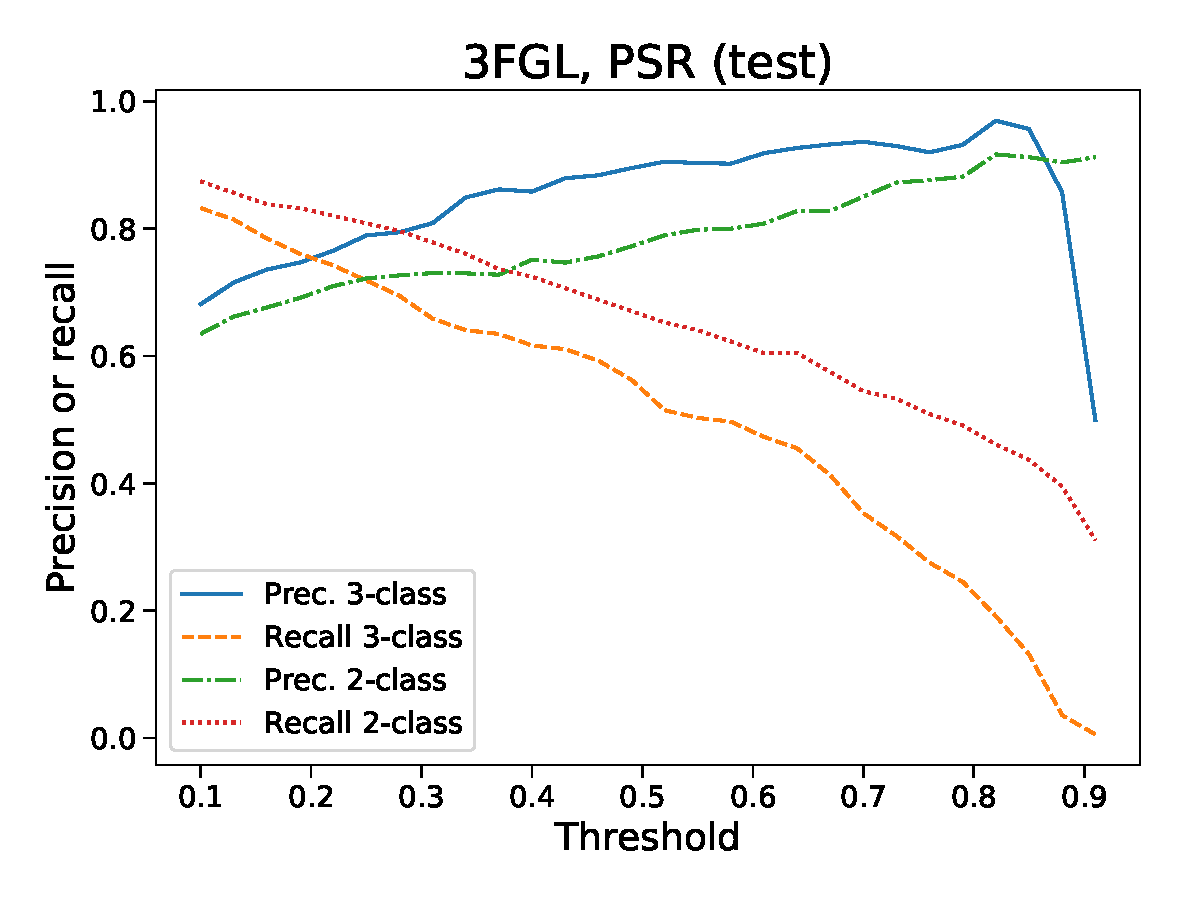
\includegraphics[width=0.45\textwidth]{plots/thresholds/thresholds_prec_recall_3FGL_PSR.pdf}
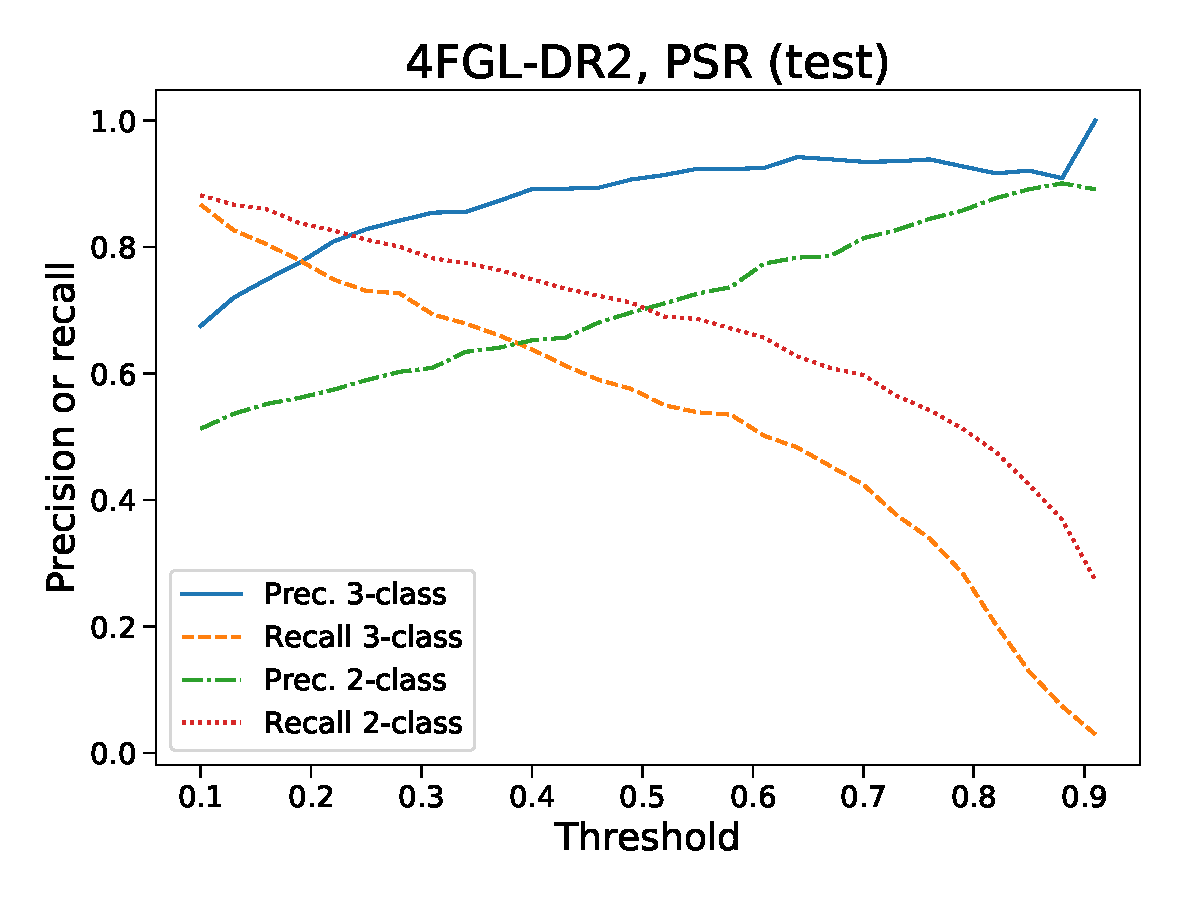
\includegraphics[width=0.45\textwidth]{plots/thresholds/thresholds_prec_recall_4FGL-DR2_PSR.pdf} \\ 
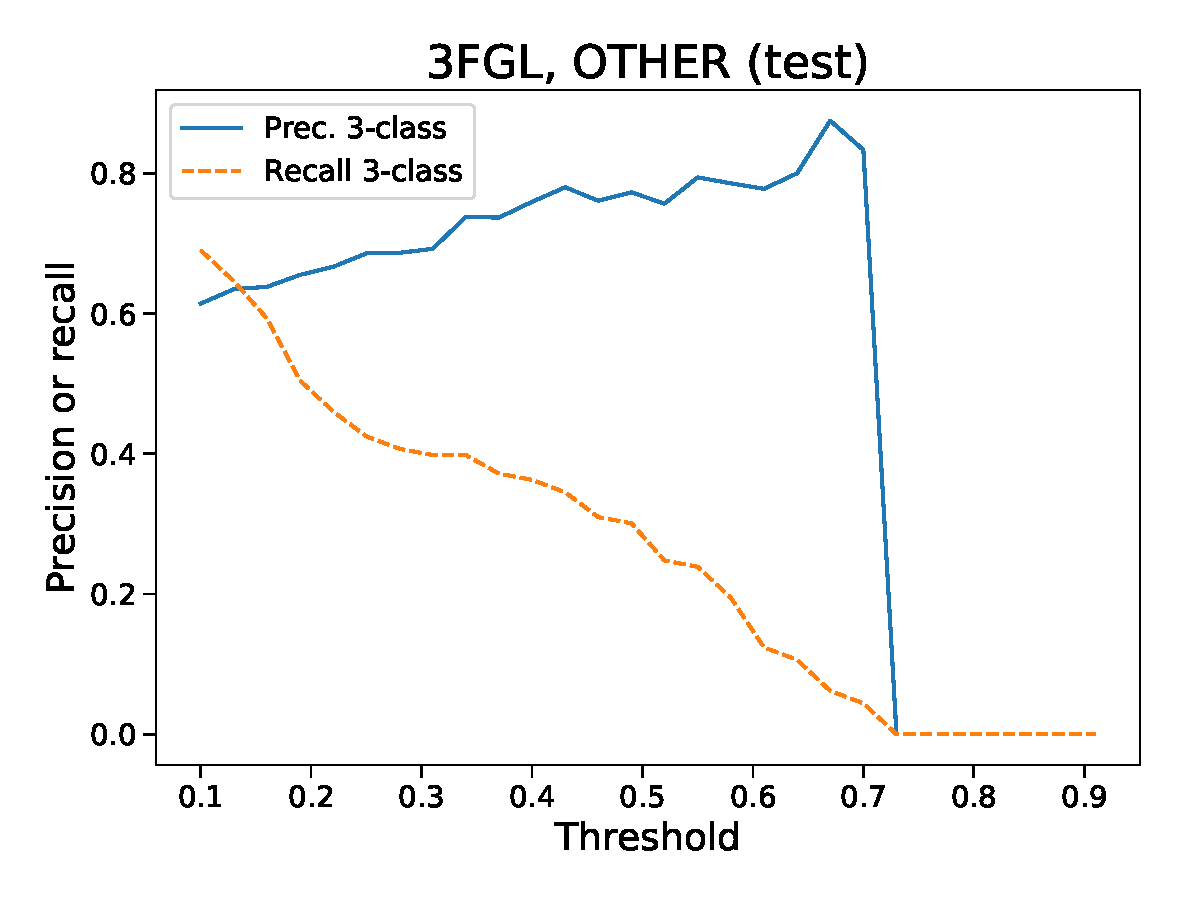
\includegraphics[width=0.45\textwidth]{plots/thresholds/thresholds_prec_recall_3FGL_OTHER.pdf}
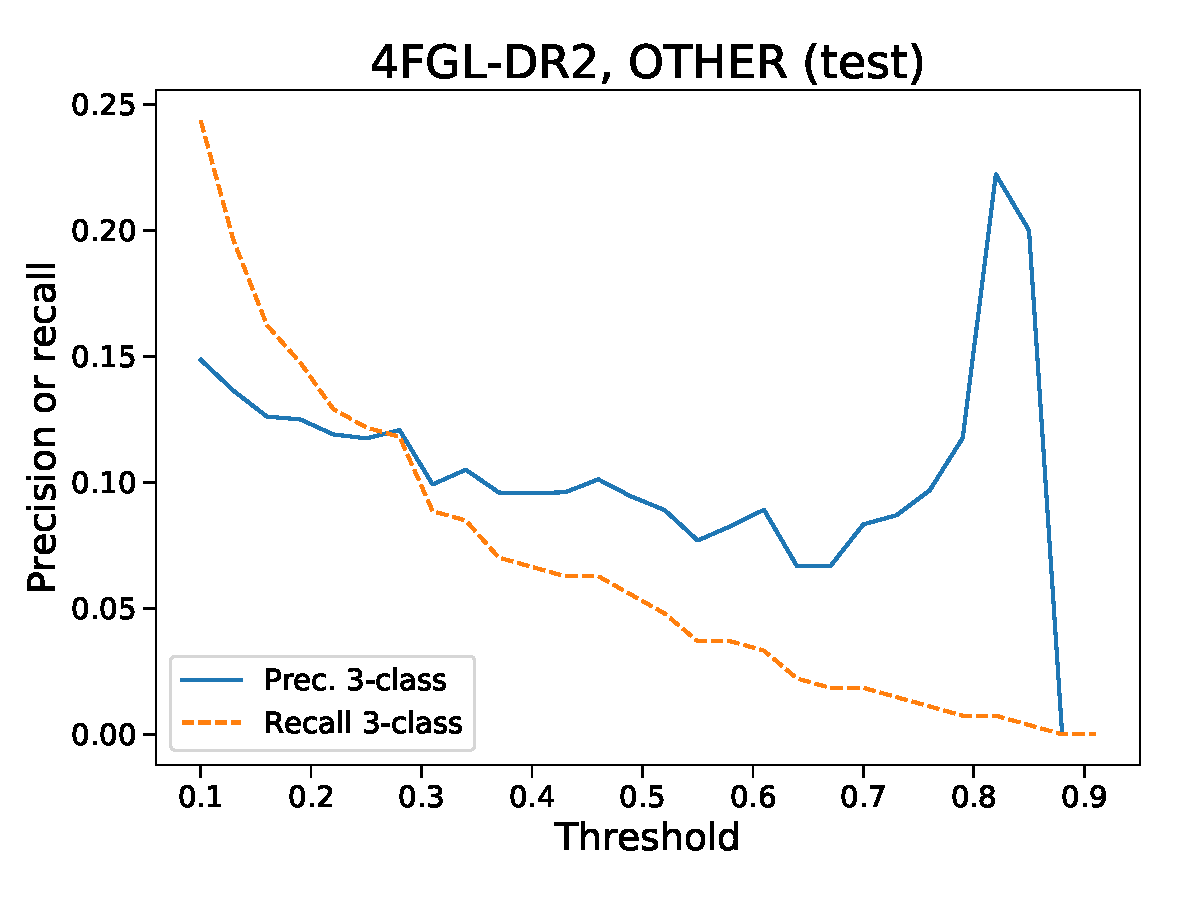
\includegraphics[width=0.45\textwidth]{plots/thresholds/thresholds_prec_recall_4FGL-DR2_OTHER.pdf}
	%\hspace*{-0.5cm}
%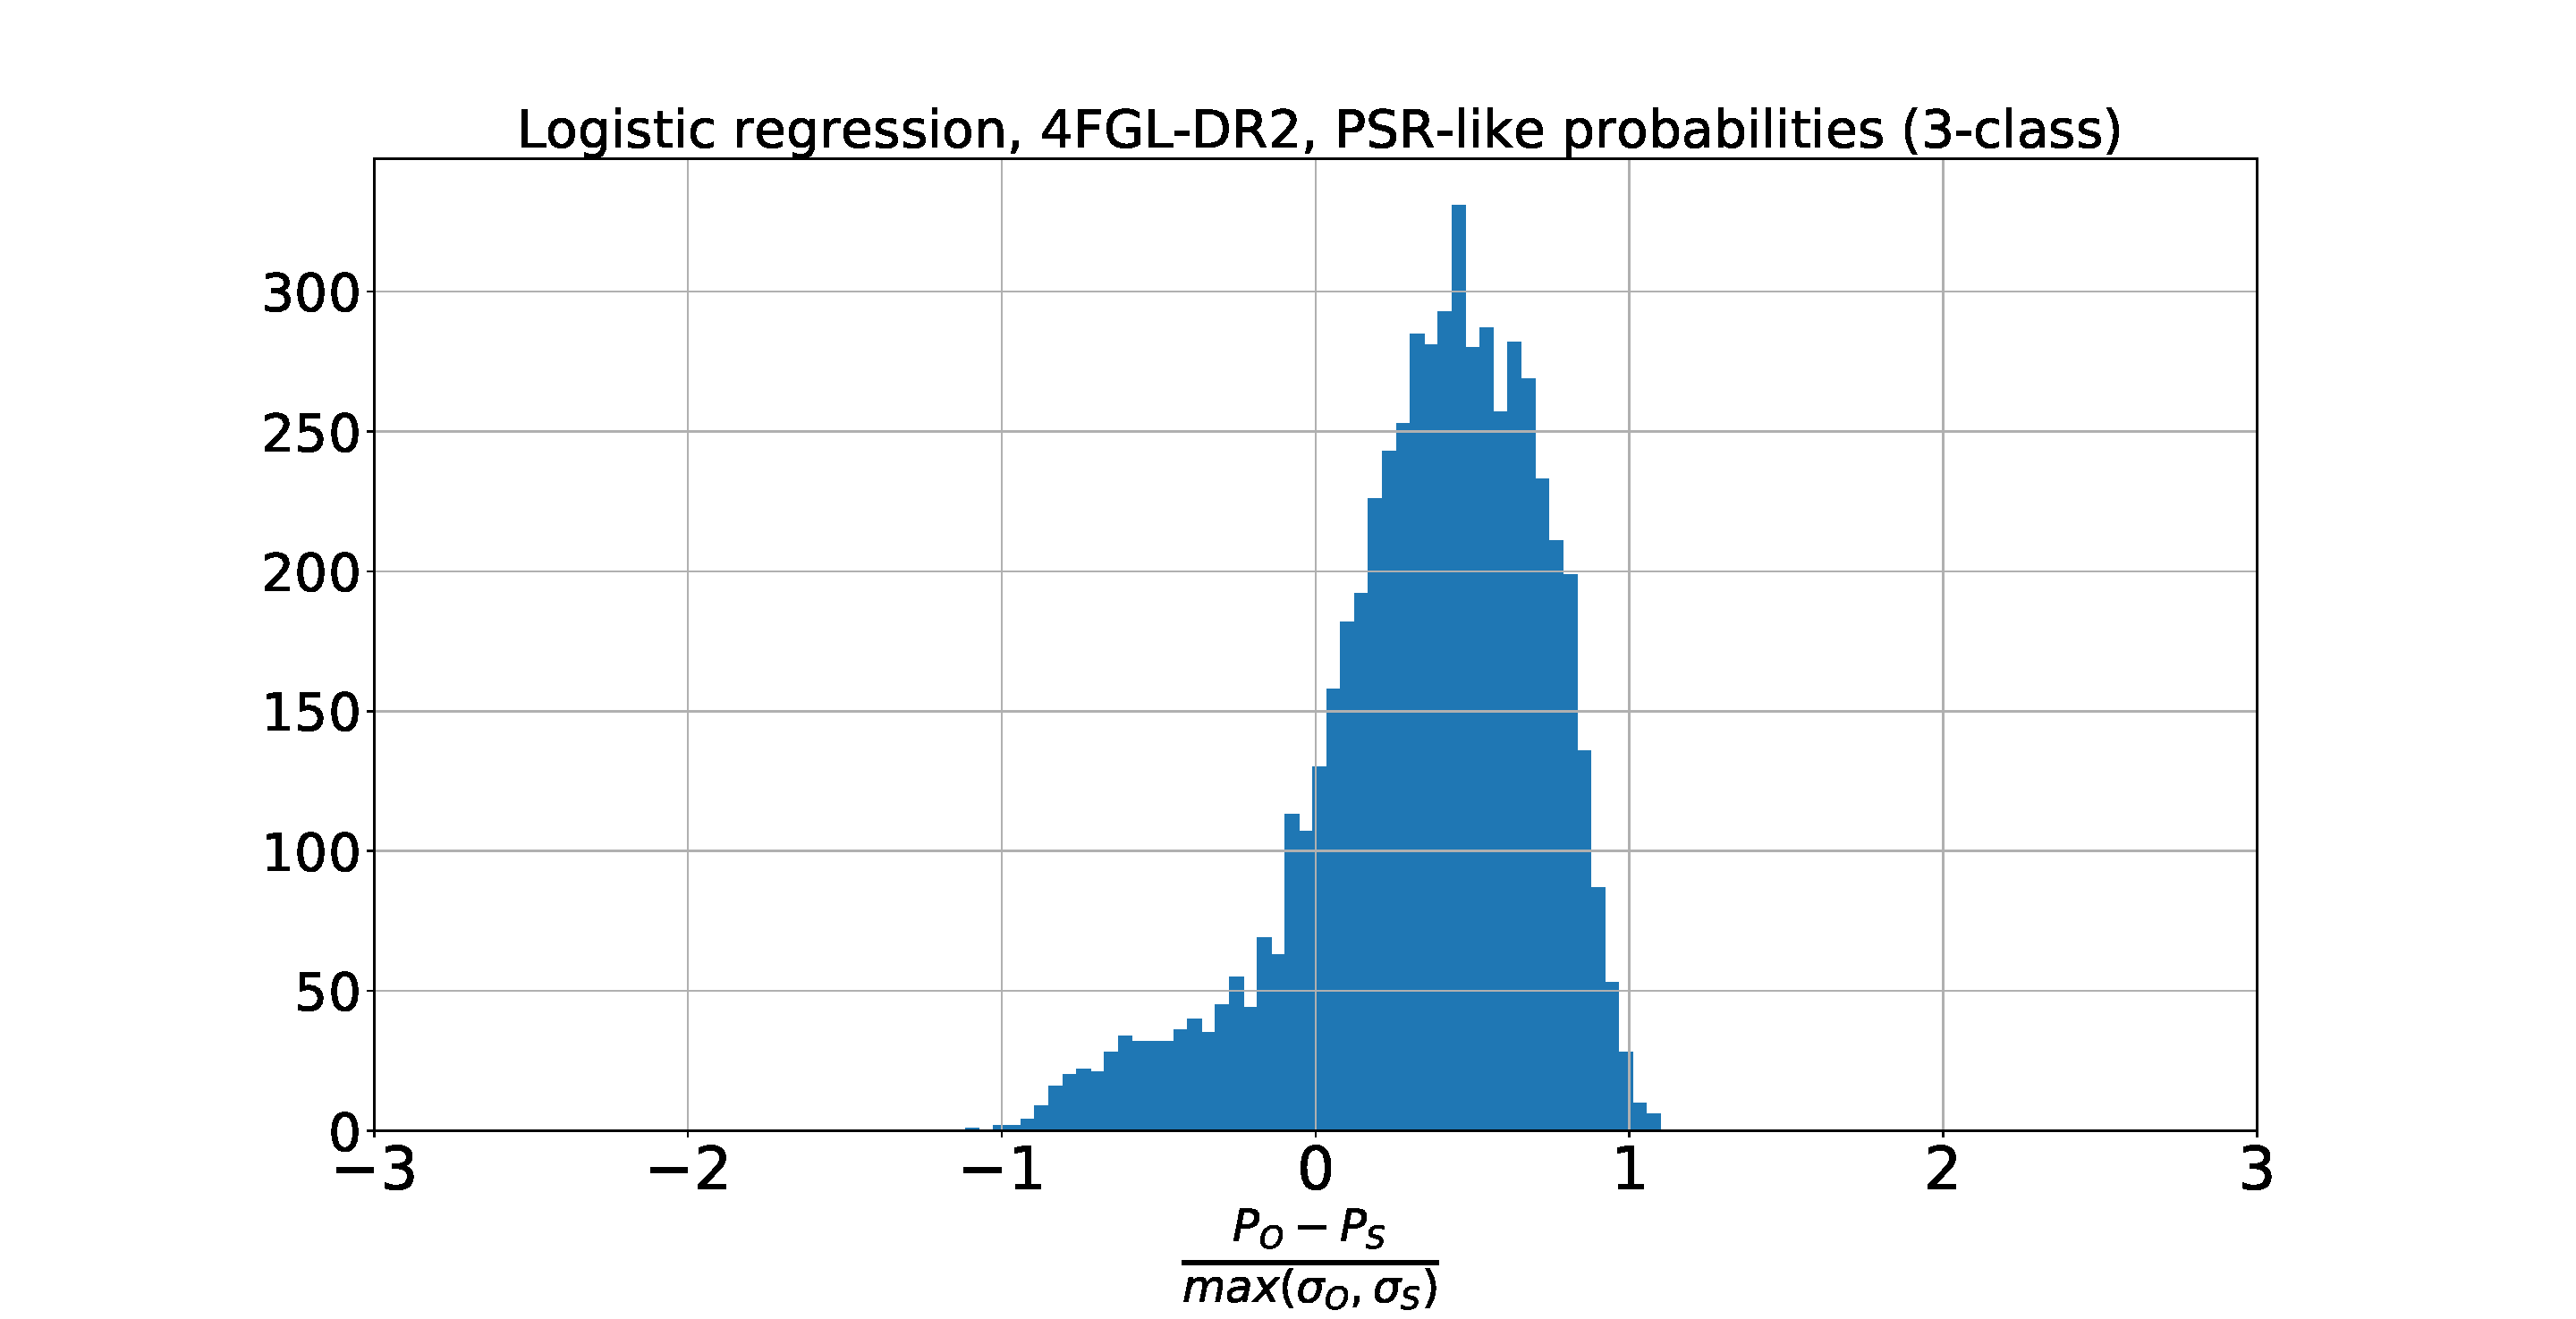
\includegraphics[width=0.55\textwidth]{plots/hist_diff_smote_LR_4FGL-DR2_3class.pdf}
\caption{Precision and recall for different choices of the threshold for classification of sources by individual algorithms.
The all-algorithms-agree method is used for the final classification. 
In these estimates, we use associated sources, the corresponding class probabilities are calculated by averaging over the probabilities when the sources are included in testing samples. Above the threshold of 0.73, no sources were classified as OTHER in the 3-class classification of the 3FGL sources. The corresponding points in the precision curve on the bottom left panel are absent.
}
\label{fig:thres}
\end{figure*}


\begin{figure*}[h]
\centering
\hspace*{-0.5cm}
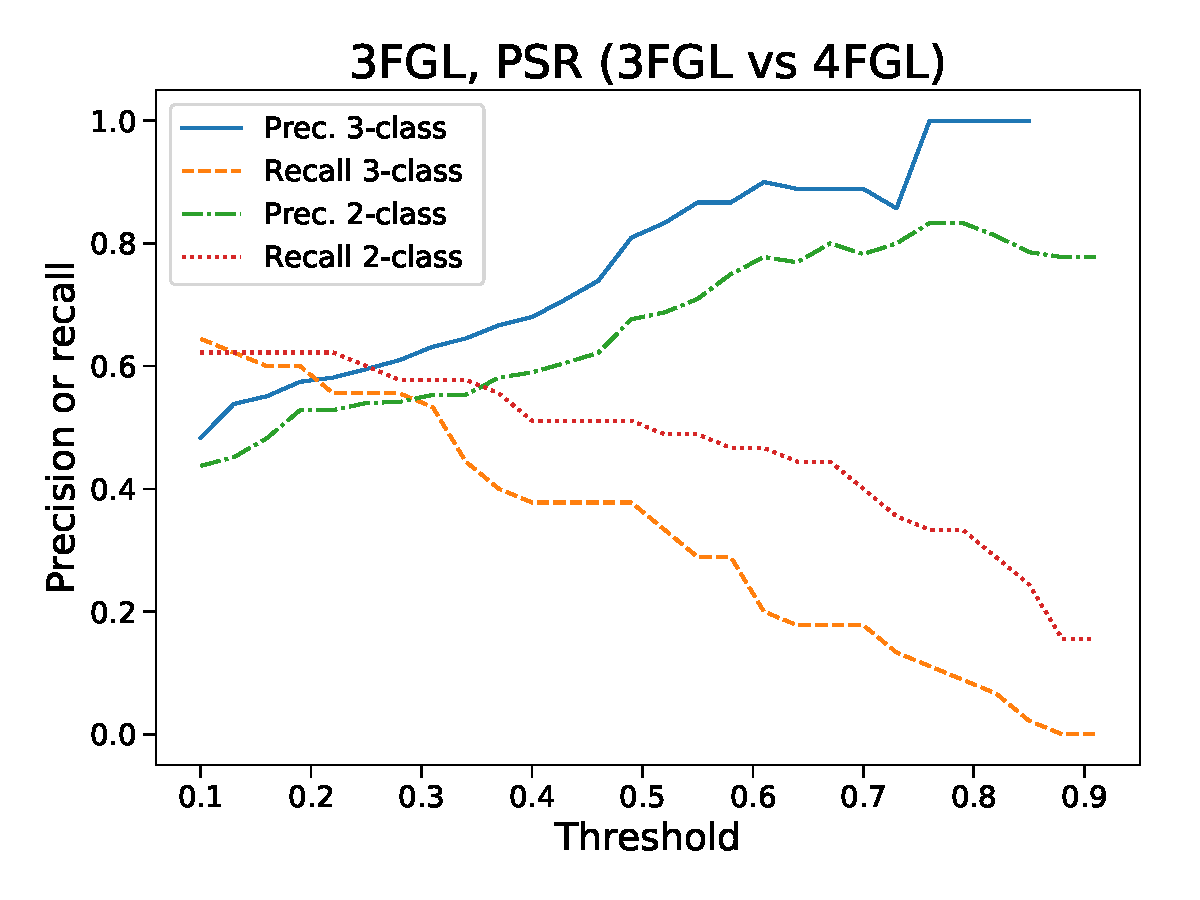
\includegraphics[width=0.45\textwidth]{plots/thresholds/thresholds_prec_recall_3FGL_vs_4FGL-DR2_PSR.pdf}
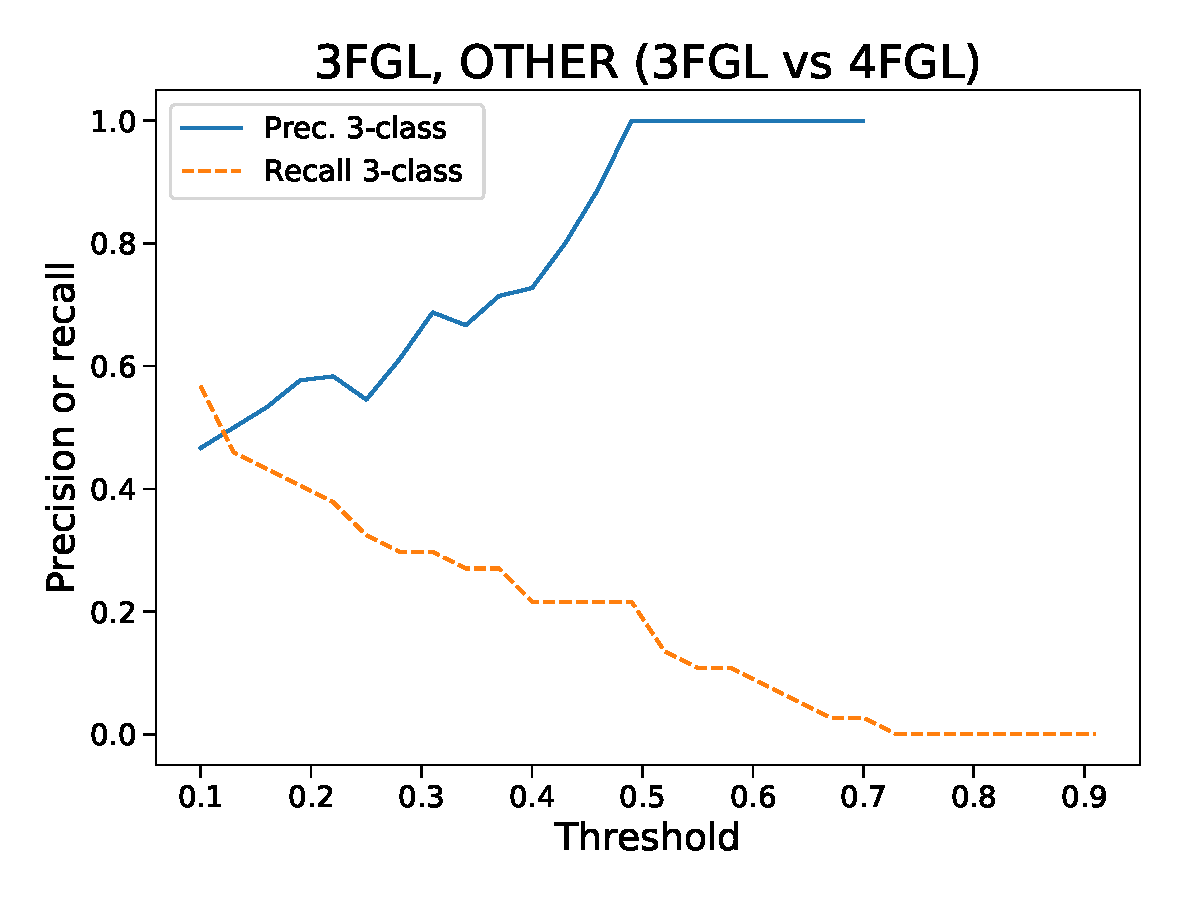
\includegraphics[width=0.45\textwidth]{plots/thresholds/thresholds_prec_recall_3FGL_vs_4FGL-DR2_OTHER.pdf}
	%\hspace*{-0.5cm}
%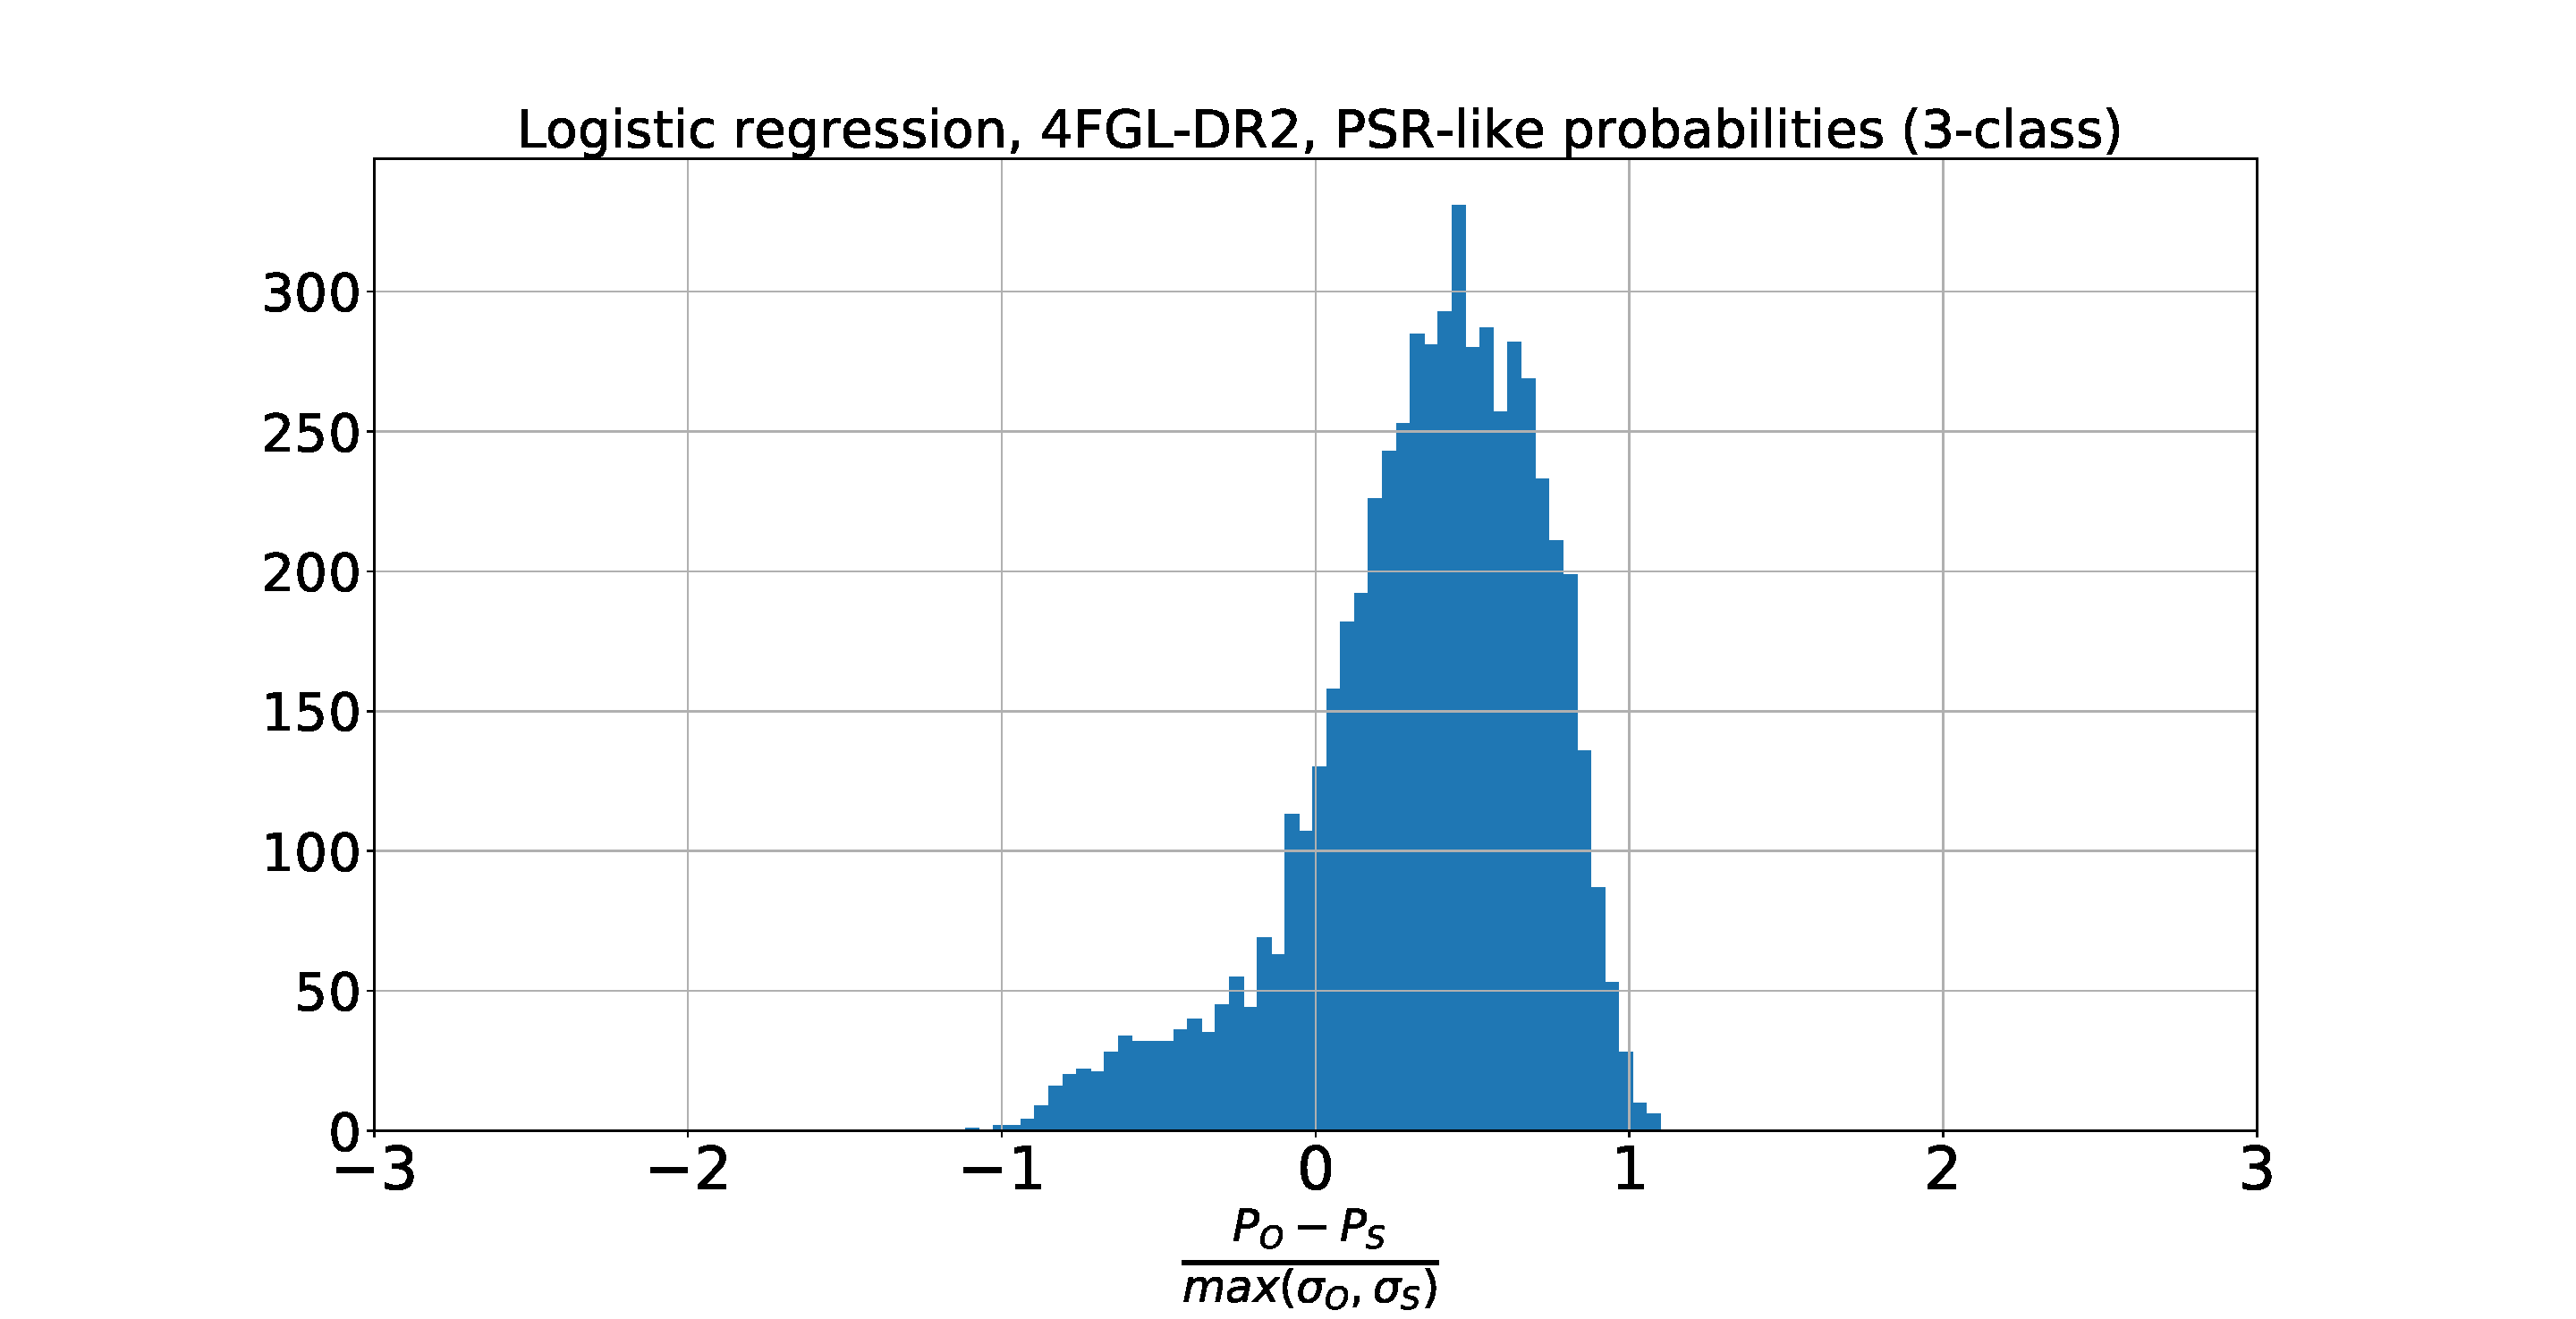
\includegraphics[width=0.55\textwidth]{plots/hist_diff_smote_LR_4FGL-DR2_3class.pdf}
\caption{Precision and recall for different choices of the threshold for classification of sources by individual algorithms.
The all-algorithms-agree method is used for the final classification. 
The precision and recall are calculated for unassociated 3FGL sources, which have associations in the 4FGL-DR2 catalog.
The classes in the 4FGL-DR2 catalog are considered as the true classes.
The points on some precision curves are absent for high thresholds, when there are no sources classified as pulsars (OTHER) on the left (right) panel in the 3-class case.
}
\label{fig:thres_3_vs_4}
\end{figure*}

In the paper we use the largest probability rule to classify sources by individual algorithms,
in particular, it means that in the 2-class case a source is classified as an AGN or a pulsar if the corresponding probability
is larger than 50\%.
Although the classification by the largest probability is a common approach in machine learning and we use it
for the calculation of accuracy of individual algorithms and for the optimization of the meta-parameters, 
one can choose other thresholds for the classification depending on the goals of the analysis.
For instance, if a list of high-probability pulsars is required, one could use a higher threshold, 
which is expected to reject most of the false candidates but real pulsars would be rejected as well, 
i.e., generally one expects a higher precision for higher threshold
at the expense of lower recall.
On the other hand, lower threshold would increase the recall (one would miss fewer true candidates), 
but decrease the precision (there will be more false positives).



In this appendix we study the effect of changing the threshold on the probabilistic classification of sources by the individual
algorithms on the overall precision and recall of classification using the agreement of all 8 algorithms.
In Figure \ref{fig:thres} we show precision and recall for the 2- and 3-class classification cases of 3FGL and 4FGL-DR2 PSR and OTHER sources.
In the calculation we use the probabilistic classification of associated sources described in Section \ref{sec:3FGLprediction1},
i.e., we perform 1000 random splits into training and testing samples and determine the class probabilities for a source by averaging the probabilities when the source is included in the test samples.
We note that with increasing threshold the recall is decreasing while the precision is generally increasing  (except for a few high threshold values in the 3FGL PSR and OTHER 3-class classification, where the number of candidates is very small).
The precision in the 3-class case is generally better than in the 2-class case (see the top panels of Figure \ref{fig:thres}),
while recall is better in the 2-class case.
There are a few points for high threshold values where no associated 3FGL sources were classified as OTHER.
In this case the precision is undetermined due to division by zero and the corresponding points are absent in the precision curve
on the lower left panel of Figure \ref{fig:thres}.


In Figure \ref{fig:thres_3_vs_4} we show the precision and recall for different thresholds for classification of unassociated sources in the 3FGL catalog, which have associations in the 4FGL-DR2 catalog. In general the precision and recall in this case are smaller than the estimates in Figure \ref{fig:thres}.  The estimates in Figure \ref{fig:thres_3_vs_4} are likely more realistic than in the test samples case, since they also take into account possible difficulties in reconstructing the properties of the sources, such as the spectrum, which can affect the probabilistic classification of the sources.




